\documentclass[11pt]{article}
\usepackage{amssymb}
\usepackage{graphicx}

\usepackage[outdir=./]{epstopdf}
\usepackage{etoolbox}
%\patchcmd{\maketitle}{\newpage}{}{}{}

%\DeclareGraphicsExtensions{.eps}

\usepackage{mathtools}
\usepackage{enumerate}
\usepackage{apacite}
\usepackage{listings}
\usepackage{multirow}
\usepackage{todonotes}
\usepackage{svg}
\usepackage{booktabs}
\usepackage{afterpage}
\usepackage{titlesec}
\titleformat*{\section}{\large\bfseries}

\usepackage[margin=1.25in]{geometry}

\newcommand{\den}[2][]{
\(
\left\llbracket\;\text{#2}\;\right\rrbracket^{#1}
\)
}


\newcommand{\KL}[2]{\ensuremath{D_{KL}({#1}\, \| \, {#2})}}
\newcommand{\E}[2]{\ensuremath{\mathbb{E}_{#1}\left [#2 \right]}}

\newenvironment{figurehere}
	{\def\@captype{figure}}
	{}

\setcounter{tocdepth}{2}
\usepackage{lipsum}
%\pagenumbering{gobble}
%\usepackage{apacite}

%\linespread{1}
\usepackage{textcomp}
\usepackage{lingmacros}
\usepackage{setspace}%\doublespacing 

\DeclareGraphicsRule{.tif}{png}{.png}{`convert #1 `dirname #1`/`basename #1 .tif`.png}
\graphicspath{{./figures/}}
 
%\makeatother

\title{Pr\'ecis of \emph{Coordinating on meaning in communication} }
\author{Robert D. Hawkins \\ \small Department of Psychology, Stanford University}
\date{}

\begin{document}
%\thispagestyle{otherpage}

\maketitle

It is tempting to think of word meanings as entries in a dictionary shared by speakers of a language. 
Drop into any conversation between friends, however, and you wade into a stream of shorthand, jargon, slang, references, nicknames, and inside jokes --- some of which you may understand, but the rest of which may be meaningful to them alone. 
There is no guarantee, it seems, that any two speakers of a language will share the same dictionary.
To make matters worse, we live in an ever-changing world where we need to talk about new things.
There is also no guarantee that any dictionary could anticipate the meanings we will need to express in each new context.
If we cannot rely on the existence of a shared dictionary for coordination, what can we rely on?
How do we manage to understand one another so effortlessly in this patchwork landscape of meaning?

My dissertation investigates the cognitive mechanisms that allow individuals, and communities, to solve this challenge.
The core theoretical contribution is an account of communication relaxing the assumption that speakers of a language share the same ``protocol.''
Instead, we propose that communication is better understood as a multi-agent meta-learning problem guided by social inference.
Agents must integrate background expectations about reliable community-wide conventions with new \emph{ad hoc}, partner-specific pacts constructed on the fly.
Chapters 2 formalizes this proposal in a hierarchical Bayesian model and presents simulation results capturing key effects from the literature. 
Chapter 3 evaluates an algorithm scaling this proposal to a recurrent neural network that interactively adapts to human partners using natural language.
Chapter 4 introduces a large behavioral corpus that provides a higher resolution look at the dynamics of \emph{ad hoc} convention formation. % of referring expressions in the classic Tangrams task. 
Chapter 5 tests how the communicative needs of the context shape the resulting \emph{ad hoc} conventions. 
Finally, Chapter 6 assesses the generality of the proposed mechanisms by examining convention formation in a \emph{graphical} Pictionary task. 

Understanding the role of learning and social cognition in everyday language use is a foundational question at the intersection of psychology, neuroscience, and linguistics. 
The methodological combination of computational modeling and naturalistic communication experiments gives new insight into how such rich, flexible language behavior may arise from these general-purpose cognitive mechanisms.
The proposed theory builds on accounts of social convention and meaning developed in analytic philosophy, particularly by \citeA{Lewis69_Convention} and \citeA{davidson_nice_1986}, and suggests broader application potential toward building more adaptive and socially intelligent AI, consistent with current directions in computer science. 
More broadly, this work opens avenues for future work to understand how social conventions and norms are represented in the mind, how these conventions are shaped by local context, and how they give rise to the remarkable feats of social coordination that are so distinctive of human cultures \cite{hawkins2019emergence}.

\section*{Introduction}

A core function of communication is \emph{reference}: using words to convey the identity of an object in the environment \cite{Brown58_HowShallAThingBeCalled,Searle69_SpeechActs,van_deemter_computational_2016}.
Throughout my dissertation, I use a rich, naturalistic communication paradigm called a \emph{repeated reference game} \cite{KraussWeinheimer64_ReferencePhrases} that requires a pair of participants to find some way of referring to novel, ambiguous stimuli they don't already have strong conventions for.
%In this task, pairs of participants are presented with arrays of novel images.
On each trial, one participant (the director) is privately shown a \emph{target} object in an array of distractors and must produce a referring expression allowing their partner (the matcher) to correctly select that object from the array. 
Critically, each object appears as the target multiple times in the trial sequence, allowing the experimenter to examine how referring expressions change as the director and matcher accumulate a shared history of interaction, or `common ground' \cite{clark_using_1996}.
To the extent that the director and matcher converge on a stable and accurate system of referring expressions, and these referring expressions differ from the ones that were initially produced, it may be claimed that \emph{ad hoc conventions} or \emph{pacts} have been constructed within the dyad.

One of the earliest and most intriguing phenomena observed in this task is that descriptions are dramatically shortened across repetitions: an initial description like ``the one that looks like an upside-down martini glass in a wire stand'' may gradually converge to ``martini'' by the end.
That is, speakers are able to communicate the same referential content much more efficiently over time.
Subsequent work has established a number of signature properties of this process through careful experimental manipulation.
First, the extent to which descriptions are shortened is \emph{contingent} on evidence of understanding from the matcher \shortcite{KraussWeinheimer66_Tangrams,KraussEtAl77_AudioVisualBackChannel,HupetChantraine92_CollaborationOrRepitition}, and is therefore not easily explained as a mere practice or repetition effect.
Second, the resulting labels are \emph{partner-specific} in the sense that they do not transfer if a novel matcher is introduced \shortcite{WilkesGibbsClark92_CoordinatingBeliefs,MetzingBrennan03_PartnerSpecificPacts,brennan_partner-specific_2009}.
Third, they are \emph{sticky} in the sense that they persist through precedent with the same partner even after the referential context changes \cite{BrennanClark96_ConceptualPactsConversation}, and are readily extended to similar objects \cite{MarkmanMakin98_ReferentialCommunicationCategory}.

These qualitative effects provide a core empirical backbone for theories of communication to explain, but immediately pose difficulties for current computational models.
One of the most promising candidates is a family of probabilistic models which derive flexibility in meaning from \emph{de novo} Gricean reasoning, formalized as recursive social inference \cite{GoodmanFrank16_RSATiCS,FrankeJager16_ProbabilisticPragmatics}.
These models show how listeners use context to draw enriched inferences about intended meaning even in cases of ambiguous or non-literal usage \cite{Clark83_NonceSense,LascaridesCopestake98_PragmaticsWordMeaning,Glucksberg01_FigurativeLanguage}.
While such one-shot pragmatic reasoning has provided a powerful explanation of many forms of flexibility, it remains insufficient to explain the dynamics of how new meanings become shared \emph{over time}.
Like other models of communication descended from \citeA{Shannon48}, the problem is that recursive reasoning still bottoms out in a fixed  `dictionary' of literal meanings assumed to be already shared between speakers.
To overcome this problem, I turned to the literature on language acquisition and language evolution, which focus on how meaning arises in the first place.
I suggest that the same learning mechanisms may play a ubiquitous role in establishing meaning even in ordinary interactions between adults. 

%Recent probabilistic modeling framework which derives pragmatic considerations of language use from more generic computational principles of social cognition in rational agents.
%%, specifically recursive probabilistic inference about the beliefs and intentions of rational agents. 
%% \emph{Gricean pragmatics} due to their origins in Paul Grice's ``cooperative principle,'' operate within the production or comprehension of a single utterances. 
%For example, listeners treat the literal meaning of a question as a cue to infer and address the underlying goal of the questioner \cite{hawkins_why_2015, hawkins_QA_2018}.
%And even though many labels may be literally true of an object, speakers refer to objects at an appropriate level of specificity given the other objects in context \cite{graf_animal_2016, monroe2017colors}.
%They also increase the specificity of their utterances under additional uncertainty over what else might be in their partners' visual field \cite{hawkins_conversational_2016, hawkins2018speakers}.

%Here we lay out the theoretical landscape and empirical evidence focusing on three key aspects of our theoretical approach: 
%\begin{enumerate}
%\item  the context-sensitive semantic priors that represent our initial uncertainty over what a novel partner is likely to mean by a word, 
%\item the path-dependence and increasing efficiency of our communicative behavior across even short periods of repeated interaction, and 
%\item the pattern of generalization from learning local interactions to new contexts and new partners. 
%\end{enumerate}

%The core of this work is an inferential model of convention formation that explains flexible and adaptive language use across extended interaction as a consequence of hierarchical probabilistic learning. Through observing their partner's usage, agents attempt to infer and adopt their partner's underlying lexicon using global conventions as a prior. When both agents independently adopt such a learning strategy, they align to one another, coordinating on and implicitly creating new, shared conventions. 

\begin{figure}[t!]
\centering
\includegraphics[scale=.85]{chapter2}
\caption{\small Model and simulation results from Chapter 2. (A) Schematic of hierarchical Bayesian model. (B) Accuracy rises as speaker and listener coordinate. (C) Utterances reduce as speaker becomes more confident of partner's meaning. (D) Model initially represents meanings as partner-specific but generalizes convention after several partners use same meanings.}
\label{fig:chapter2}
\end{figure}

\section*{Chapter 2: An inferential model of convention formation}

A key difficulty of rejecting the assumption of a shared `dictionary' is that adults \emph{do} nonetheless bring strong background expectations about meanings into their interactions. 
After all, these expectations are precisely the end-point that models of language acquisition and language evolution seek to explain, over different timescales.
How can agents both maintain stable beliefs about what will be meaningful to new partners, and also flexibly deviate from these meanings on a partner-specific basis?
This apparent tension between stability and flexibility suggests three functional desiderata for computational models of meaning:

\begin{enumerate}
\item a mechanism for how community-wide \emph{conventions} \cite{Lewis69_Convention} shape initial interactions with a new partner.\vspace{-.75em}
\item a mechanism for how new \emph{ad hoc} conventions can be so rapidly constructed with an individual partner.\vspace{-.75em}
\item a mechanism connecting the two: how and when are meanings generalized from individuals to communities?
\end{enumerate}

In \textbf{Chapter 2}, I propose a hierarchical Bayesian model (HBM) of convention formation and argue that it satisfies these three desiderata. 
HBMs have been key to understanding how the human mind solves a range of other difficult inductive problems where abstract, shared properties must be jointly inferred with idiosyncratic particulars of instances, including causal learning \cite{KempGoodmanTenenbaum10_LearningToLearn,GoodmanUllmanTenenbaum11_TheoryOfCausality}, speech perception \cite{KleinschmidtJaeger15_RobustSpeechPerception} and concept learning \cite{KempPerforsTenenbaum07_HBM}. 
In the context of communication, the first step is to replace the shared `dictionary' of meanings with a distribution representing ``lexical uncertainty'' over different possible dictionaries a particular partner might be using \cite<see>{CooperEtAl15_ProbabilisticTypeTheory,BergenLevyGoodman16_LexicalUncertainty,SmithGoodmanFrank13_RecursivePragmaticReasoningNIPS,PottsEtAl16_EmbeddedImplicatures}.
In an HBM, this uncertainty is assumed to be hierarchically structured (see Fig. \ref{fig:chapter2}A).
The top level is a stable prior representing abstract conventions shared across all agents in the community, while idiosyncratic partner-specific knowledge is represented at the lower level.
This roughly corresponds to the distinction made by \citeA{davidson_nice_1986} between a ``prior theory'' and a ``passing theory.''
In other words, conventions supply a useful but often uncertain first guess about the linguistic meanings that will be shared with a new partner.

Critically, these expectations may then be updated using evidence of a partner's language use.
Specifically, agents use Bayesian theory of mind to make inferences about that partner's latent `dictionary,' leading to local \emph{ad hoc} conventions.
As each party learns about the other and attempts to be understood under their updated model of partner-specific meaning, they may coordinate on a system of meaning that is tailored to be efficient and accurate for their present purposes.
Thus the shared semantic prototype can be thought of as a backbone supporting rapid learning for new partners and situations, and may in turn be learned by pooling across many extended interactions with individuals.
In summary, this model formalizes a functional view of linguistic conventions as solutions to a meta-learning problem, in which every agent is simultaneously seeking to infer and use the conventions that other agents are using, to support more successful communication. 
%This model can be contrasted Rather than priming or aligning on surface forms, these agents are making structured inferences about the underlying representation of meaning used by their partner.

%In \textbf{Chapter 2}, we propose a hierarchical Bayesian model of convention formation that formalizes our proposal (see Fig. \ref{fig:modelschematic}): global conventions are learned and generalized over many extended interactions with many different people across a lifetime, and 

I evaluated this model through a series of simulations.
First, I showed that two agents updating their beliefs about meaning in this way can coordinate even in the absence of strong initial priors (Fig. \ref{fig:chapter2}B).
Their initial choices can be taken as evidence for a particular lexicon and become the basis for successful communication.
Second, I showed that a preference for less costly utterances combined with learning gives rise to shorter descriptions over time (Fig. \ref{fig:chapter2}C).
The speaker model initially produces longer utterances as a way of hedging against their own uncertainty about what meanings will be understood, but omits words over time as they become more confident. 
Third, I tested the model's pattern of generalization over different partners (Fig. \ref{fig:chapter2}D).
When a new partner is first introduced, it reverts nearly to its original state, displaying the signature phenomenon of partner-specificity. 
As it interacts with different partners using language in a similar way, however, these \emph{ad hoc} conventions gradually become bona fide \emph{community-level} conventions that are readily extended to initial encounters with new partners. 
These simulations of key qualitative phenomena suggest that the proposed HBM is a promising computational account of how conventions are represented and learned at different scales.

% assumes others are using some set of conventions and is trying to learn them such that they can be understood.  %: global conventions are learned and generalized over many extended interactions with many different people across a lifetime, and  this shared semantic prototype is the backbone supporting rapid learning for new partners and situations. 
%This model successfully predicts coordination on idiosyncratic but path-dependent and stable form-meaning mappings in simulations, and shows that 

%First, we show in simulations of a repeated interaction with a single partner that this model successfully allows coordination on arbitrary but path-dependent and stable form-meaning mappings and that a preference for less costly utterances combined with learning gives rise to reduction (see Fig. \ref{fig:modelresults}). Second, we test the generalization properties of our model by manipulating partners and contexts: 
%\begin{enumerate}
%\item how `sticky' are the pacts formed in one context (i.e. a Dalmatian in the context of other dogs) when the same target is transplanted to a new, less restrictive context (i.e. a Dalmatian in the context of a cat and bear; see Brennen \& Clark, 1996), 
%\item to what extent do agents revert to longer utterances after swapping out partners mid-way through a game (see  Wilkes-Gibbs \& Clark, 1992; Metzing \& Brennen, 2003; Yoon \& Brown-Schmidt, 2014), and 
%\item how do local, partner-specific expectations generalize to global expectation over repeated interaction with multiple partners in the same community (see Fay et al. 2010).
%\end{enumerate}

\section*{Chapter 3: Coordination between humans and machines}

\begin{figure}[t]
\centering
\includegraphics[scale=.7]{chapter3}
\caption{\small Modeling approach and experiments from Chapter 3. (A) Schematic of a regularized continual learning approach that allows artificial agents to rapidly adapt to their partner through interaction, which was evaluated using both (B) an interactive listening task where the agent interpreted referring expressions from a human speaker and (C) a speaker task where the agent produced descriptions for a human listener.}
\label{fig:chapter3}
\end{figure}

While the hierarchical Bayesian model explored in Chapter 2 is shown to have desirable theoretical properties, it also becomes intractable to use as the vocabulary and object set grows, making it untenable for modeling arbitrary natural language.
In \textbf{Chapter 3}, I instead take the community-level expectations to be an initialization for the weights of an image-captioning neural network.
Just as probabilistic models have assumed a fixed `dictionary,' approaches based on deep neural networks typically learn a monolithic meaning function during training, with fixed weights during use.
I exploit theoretical connections between the hierarchical Bayesian framework and recent  approaches to multi-task- and meta-learning in deep neural networks \cite{nagabandi_deep_2018,grant_recasting_2018,jerfel_online_2018} to propose an online continual learning approach for a neural image-captioning model.
Specifically, the community-level prior corresponds to a pre-trained, task-general initialization.
Conditioning on new data from a particular partner corresponds to regularized gradient descent (Fig. \ref{fig:chapter3}A).

To evaluate this approach, I implemented a repeated reference game using images from the validation set of COCO \cite{lin2014microsoft} as the targets of reference.
I considered the model's ability to form \emph{ad hoc} conventions with human partners in two different tasks, which presented distinct challenges for its initialized background expectations.
First, in a \emph{listening} task (Fig. \ref{fig:chapter3}B), the model is paired with a human speaker and must learn to interpret their natural referring expressions in challenging contexts.
Chatbox messages were sent to a GPU where the model weights from the previous trial were loaded, used to generate a response, and updated in real-time for the next round with a latency of approximately 6-10 seconds.
The listener model initially performs much less accurately than a baseline human listener because of the idiosyncratic and out-of-sample language produced by the human speaker.
Yet our model rapidly improves in accuracy as it fine-tunes a parthner-specific representation.
Second, in a \emph{speaking} task (Fig. \ref{fig:chapter3}C), the model is paired with a human listener and must learn to \emph{generate} appropriate referring expressions in easier contexts.
The model initially produced more complex referring expressions than required to distinguish the images, due to biases from its training corpus, but it became dramatically more efficient over the course of the interaction while maintaining high accuracy. 
These results validate the proposed inferential model of convention formation on real natural-language input and output, and suggest further avenues of application potential for adaptive artificial intelligence based on basic cognitive principles.

\section*{Chapter 4: Characterizing the dynamics of coordination} 

\begin{figure}[b!]
\centering
\includegraphics[scale=.93]{chapter4}
\caption{\small Experimental design for repeated reference game used in Chapter 4.  Participants were paired over the web and communicated freely using a chat box. After a selection is made, the director is given feedback about which object was selected, and the matcher is given feedback about the true target object. Tangram stimuli were reproduced from Clark \& Wilkes-Gibbs (1986).}
\label{fig:chapter4}
\end{figure}

%In this paradigm, two participants are placed in an interactive environment containing a chat box and an array of objects. 
%On each round of the game, one player---the speaker---is privately shown one object highlighted as the target. 
%The speaker must then produce a message allowing their partner to identify and select the target from their own screen.
%Thus, when participants are pre must coordinate with one another on a way of repeatedly referring to novel, difficult-to-describe tangram shapes. 

As theories are increasingly formalized as computational models like those in the previous chapters, finding criteria to distinguish between them will depend critically upon resolving more detailed theoretical questions about the dynamics of adaptation in natural language communication.
\textbf{Chapter 4} describes a new, open corpus ($> 15,000$ messages) of repeated reference games (see Fig. \ref{fig:chapter4}) and a variety of analyses that address current gaps in measurement and establish a firmer theoretical foundation for future modeling work.
This effort addresses two methodological challenges that have limited the ability of previous studies to provide a sufficiently fine-grained characterization of behavior.
First, more data was needed.
Recent technical developments have allowed interactive multi-player experiments to be run on the web \cite{Hawkins15_RealTimeWebExperiments}, boosting sample sizes by an order of magnitude.
%For comparison, seminal work by \citeA{ClarkWilkesGibbs86_ReferringCollaborative} used a sample of 8 pairs of participants, while the confirmatory sample alone contains 83 pairs.
Second, the computational techniques needed to work with rich natural language data were limited at the time of prior work, but have become newly tractable given developments in natural language processing (NLP).

The analyses in this chapter roughly divide into two categories, corresponding to the dynamics of syntactic \emph{structure} and semantic \emph{content}.
The investigations of syntactic structure focus on the process by which referring expressions are gradually shortened to communicate the same idea more efficiently.
One particularly simple model, for example, might predict that shortening is purely driven by a random corruption process: at each repetition, each word from the previous repetition's utterance has some probability of being dropped.
Raw word counts alone are not sufficient for disambiguating this simple model from more cognitively complex proposals.
To move beyond word counts, I extracted part-of-speech tags and syntax trees from the text to understand which parts of utterances were being dropped, and in which sequence.
In contrast to the predictions of the random corruption model, I find that clauses and modifiers tend to be dropped in clusters, preferentially leaving open-class parts of speech (e.g. an adjective and noun) by the final repetition, and that the choice to shorten an utterance or not depends on sources of listener feedback.  

Next, I examine the semantic content of utterances over the course of this shortening process.
These analyses revolve around the theoretical constructs of \emph{arbitrariness} and \emph{stability}, which have been central to accounts of convention since \citeA{Lewis69_Convention}.
Arbitrariness refers to the claim that multiple equally successful solutions exist in the space of possible conventions: there is no single optimal solution that all speakers should objectively use.
Stability refers to the claim that, once a solution has been found, speakers should not deviate from it.
I operationalize these claims in the high-dimensional space of vector embeddings for referring expressions (i.e. GloVe embeddings).
By measuring the similarity between referring expressions in this space, I find that signatures of arbitrariness and stability gradually increase over the course of the interaction.
Additionally, while different pairs coordinate on a wide range of idiosyncratic solutions to the problem of reference, they do so in a highly path-dependent manner: words that are more discriminative in the initial context (i.e. that were used for one target more than others) are more likely to persist through the final round.
Taken together, these findings characterize core processes operating within the microcosm of dyadic, natural-language interactions.

%The referring expressions generated by participants across these games reveals a number of rich qualitative phenomena about adaptation in communication. We conduct a large-scale replication of the matching task used by Clark \& Wilkes-Gibbs (1986) as well as a reference game variant with the same stimuli that allows us to track the change in referring expressions over time at a tangram-by-tangram level. We use modern natural language processing techniques to analyze the lexical and syntactic features of utterances and show (1) that the lexical pacts participants form are arbitrary and stable, and (2) that participants are reducing their referring expressions in a systematic and path-dependent manner to preserve distinctive information.

%\begin{figure}[t]
%\centering
%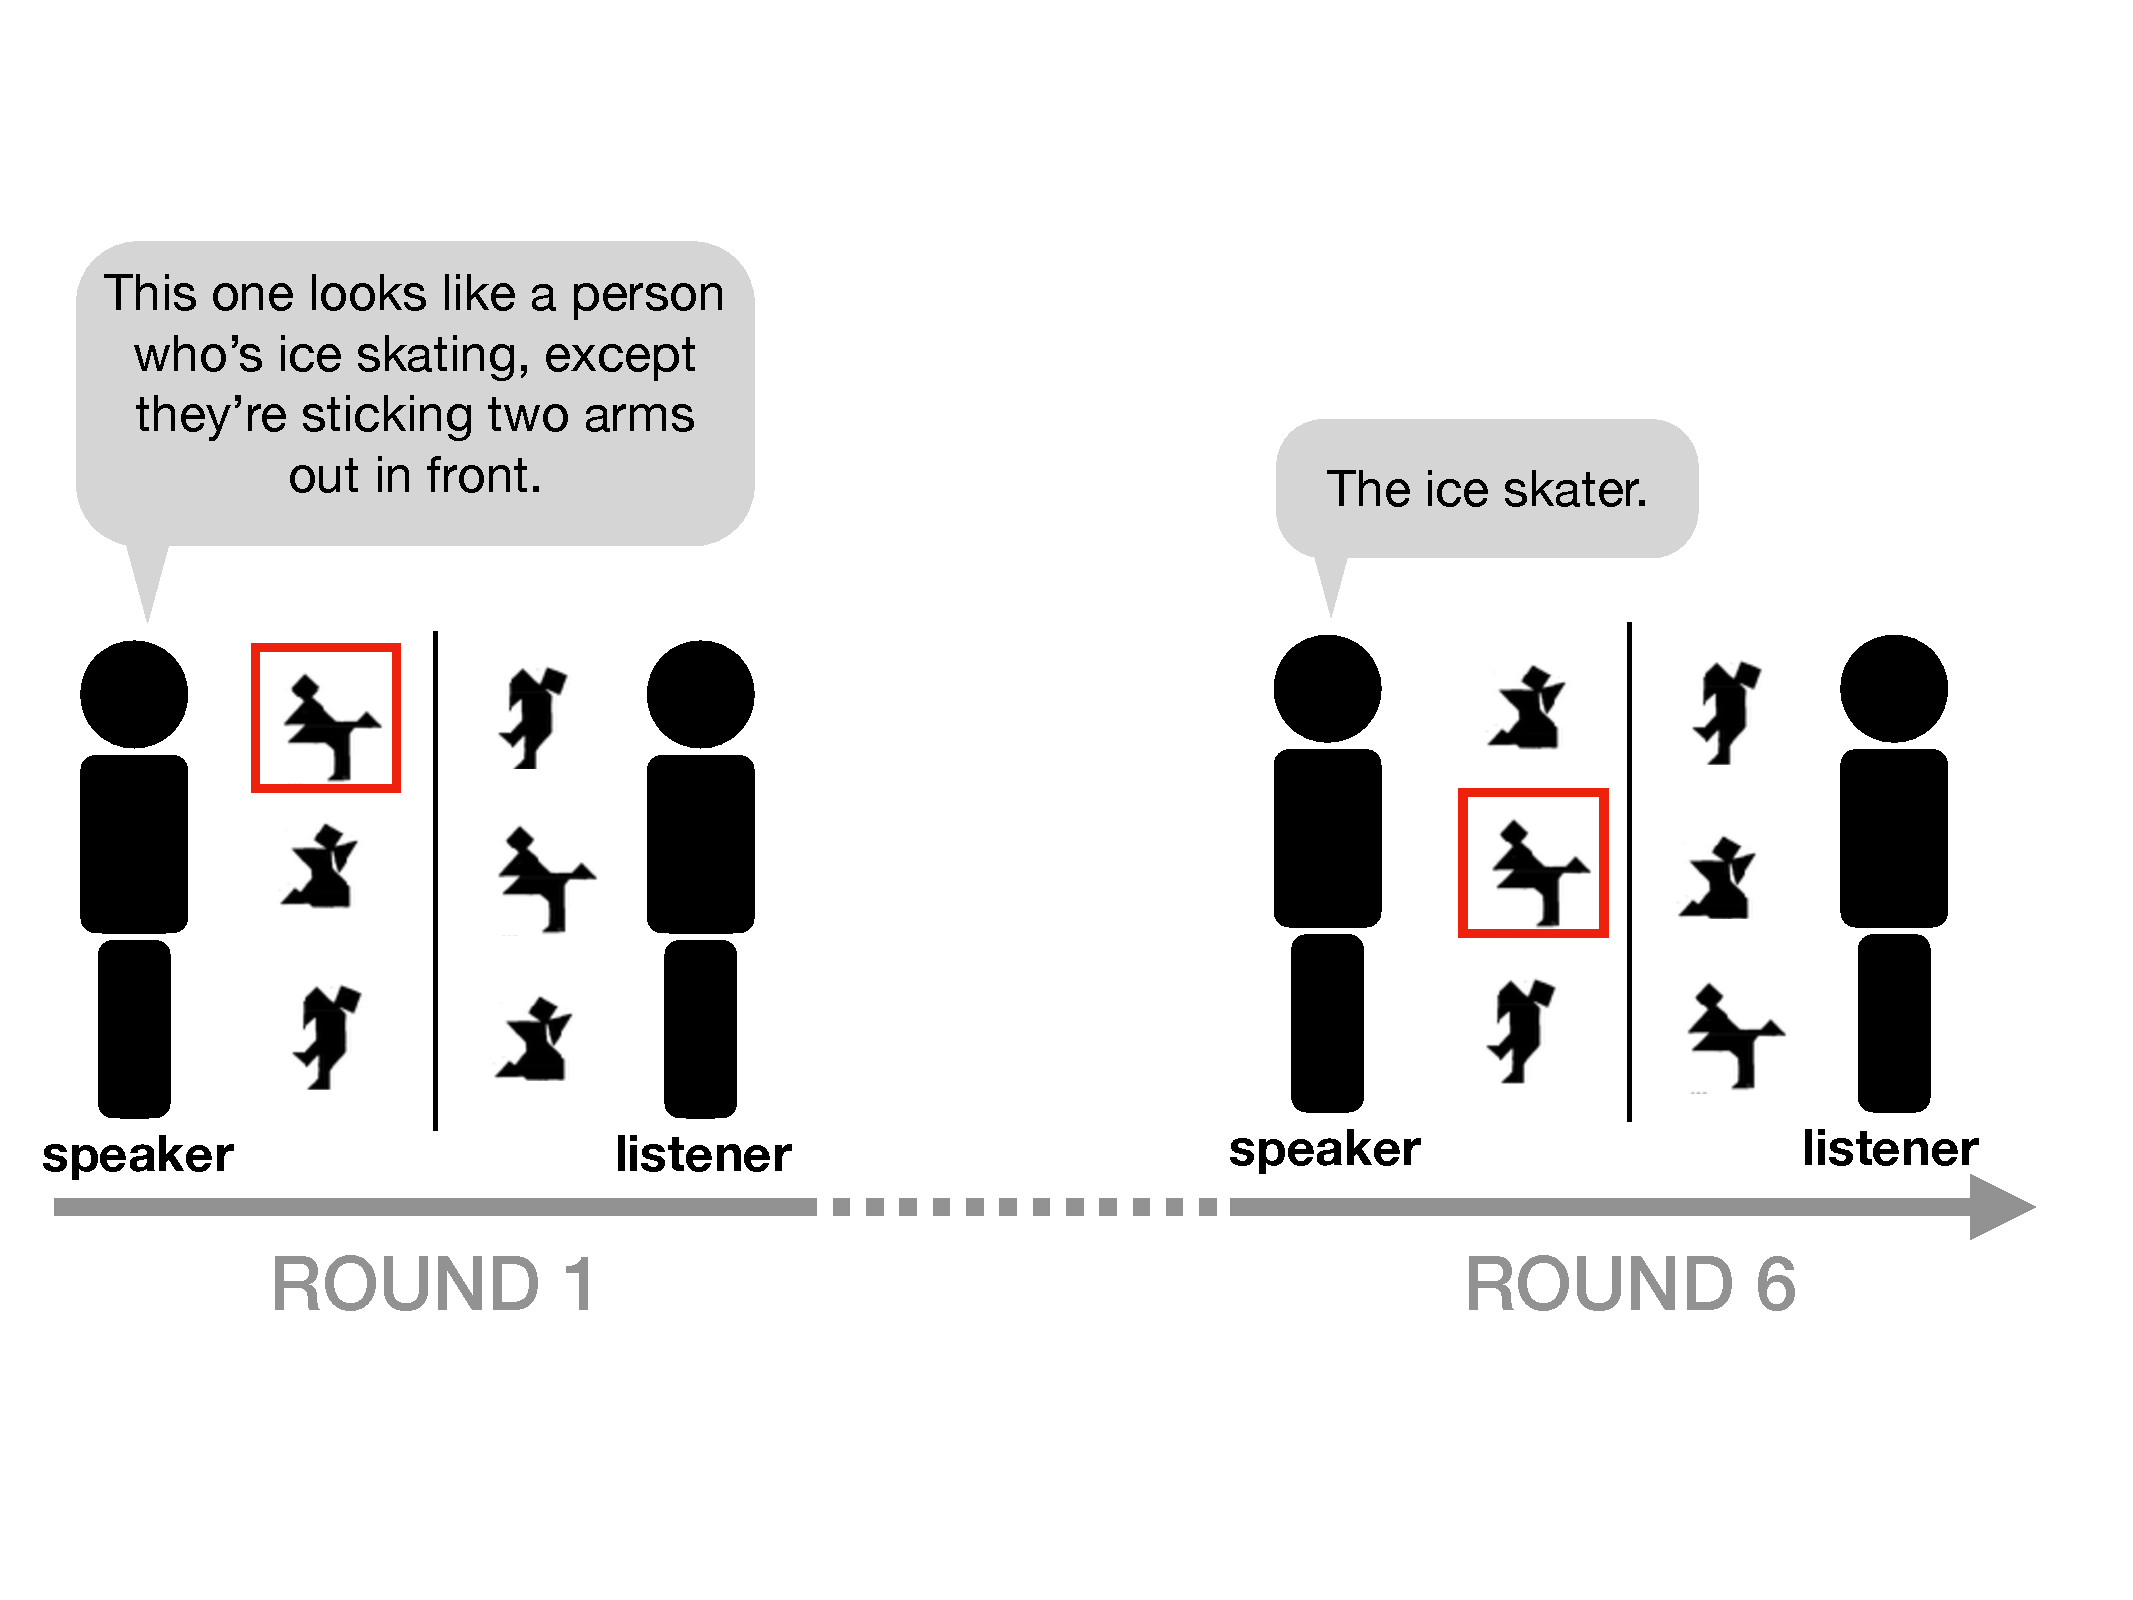
\includegraphics[scale=.45]{task_cropped.pdf}
%\caption{Generic setup for repeated reference game task in the lab using stimuli from Wilkes-Gibbs \& Clark (1986); on every round, the speaker refers to each target in some context, and the listener attempts to pick out the intended referent. Both players are free to speak at any time.}
%\label{fig:tangramsmethods}
%\end{figure}
%
%\begin{figure}[t]
%\caption{Reduction phenomena reproduced from Hawkins et al, 2017. Clockwise from left: (1) proportion of messages with subordinate clause, broken out by tangram, (2) proportion of messages with conjunction, (3) proportion of utterances containing prepositional phrase, (4) point-wise mutual information on first repetition predicts the likelihood of that word appearing in the final repetition (5) Reduction rates for different parts of speech. Error bars are bootstrapped 95\% CIs}
%\label{fig:tangramsresults}
%\end{figure}

\section*{Chapter 5: How does communicative context shape conventions?}

\begin{figure}[t!]
\centering
\includegraphics[scale=0.8]{chapter5}
\caption{\small Methods and results from Chapter 5. (A) Example of \emph{fine} context where one of the distractors belongs to the same fine-grained branch of the hierarchy as the target (i.e. another striped circle), so any abstract label would be insufficient to disambiguate them. The target is highlighted for the speaker with a black square. (B) Drag-and-drop chat box interface with artificial labels. (C) Hierarchical organization of stimuli. (D) Participants became increasingly accurate over repeated interaction. (E) Statistics of environment lead to different systems of meaning: participants developed more abstract meanings (applying to 2 objects) than specific meanings (applying to 1 object) in the coarse condition.}
\label{fig:chapter5}
\end{figure}

The rapid timescale of adaptation observed in dyadic interaction is not only of interest for cognitive theories of meaning and social coordination. 
It may also be a key building block toward understanding the remarkable adaptiveness and efficiency that is characteristic of human languages over longer time scales.
Recent computational approaches to language evolution have argued that the lexical conventions of languages balance simplicity, or learnability, with usage needs \cite{WintersKirbySmith14_LanguagesAdapt,RegierKempKay15_WordMeaningsEfficientCommunication,KirbyTamarizCornishSmith15_CompressionCommunication,gibson2019efficiency}. 
%A key prediction is that the lexicon of a language should be sensitive to the usage needs of its users. 
For example, languages in warm regions ought to be more likely to collapse the distinction between ice and snow into a single word, simply because there are fewer occasions that require distinguishing between the two \shortcite{RegierCarstensenKemp16_WordsForSnow}. 
While this is powerful explanatory principle, prior work has largely focused on the functional \emph{outcomes} of the overall language evolution process rather than the individual-level cognitive mechanisms driving the process itself.
If community-wide conventions emerge from agents generalizing across dyadic interactions, then understanding the local mechanisms leading to efficiency and informativity \emph{within} a dyad may help explain how a community’s conventions become well-calibrated to their environment. 

%A mechanistic account of lexical adaptation and convention-formation among individual agents. 

\textbf{Chapter 5} examines how the cognitive mechanisms proposed in earlier chapters allow context to shape \emph{ad hoc} conventions \cite{hawkins_emerging_abstractions_2018}.
Specifically, I propose that context-sensitivity results from the impact of inductive biases on meaning inference, specifically the Gricean expectations that a partner is trying to be appropriately informative.
To isolate these mechanisms from the background priors speakers bring into new interactions, I adopted an artificial-language paradigm from work on language evolution.
Participants were paired to communicate about a set of target objects (Fig. \ref{fig:chapter5}A) through a chatbox containing a fixed vocabulary (Fig. \ref{fig:chapter5}B) and given full feedback after each trial.
The stimuli were designed to visually cluster in a three-level hierarchy (Fig. \ref{fig:chapter5}C).
Critically, the statistics of the environment were manipulated across different pairs to make different distinctions relevant. 
In the `fine' condition, every context contained distractors that were very similar to the target, thus inducing a communicative need for finer distinctions. 
In the `coarse' condition, distractors always differed from the target at higher levels of the concept hierarchy.  
I hypothesized that pairs should coordinate on distinct names for each object when the context frequently makes fine distinctions relevant. 
Conversely, they should converge on a more efficient and compressed system of conventions for abstract categories in coarser contexts, even if a finer mapping would be sufficient.

%where when the context requires frequently making fine distinctions between entities; conversely, they should converge on a more compressed system of conventions for abstract categories (e.g. dog) in coarser contexts, even if a finer mapping would be sufficient. 
Over 100 trials, dyads were able to successfully coordinate on reliable systems (Fig. \ref{fig:chapter5}D).
Using a post-test probing the resulting conventions and a statistical approach inferring participants' beliefs about conventions at earlier stages of the task, I found systematic differences in the \emph{level of abstraction} of meanings that formed across these different conditions. 
In the coarse condition, participants learned to communicate with smaller vocabularies collapsing over distinctions within categories, while in the fine condition they coordinated on specific labels for sub-categories (Fig. \ref{fig:chapter5}E).
These differences arose even though both groups referred to each target object the same number of times; the only difference was the identity of distractors.
%Additionally, using  of the game to probe the trajectory of emergence.
These results indicate that lexical conventions are shaped by pragmatic considerations of \textit{informativity in context} as each speaker attempts to infer what the other intends to mean.
%For example, listeners can infer that the speaker would be unlikely to intend an abstract meaning like `the red squares' in a fine context: it would be underinformative and uncooperative. 
%Conversely, a speaker in the coarse condition can be confident about extending a word previously used for the dark red square to the light red square because their partner is unlikely to be confused by the presence of the original object. 
Our minds organize the world into meaningful conceptual hierarchies but our shared language may only come to reflect this structure when it is communicatively relevant. 


%\begin{figure}[h]
%\centering
%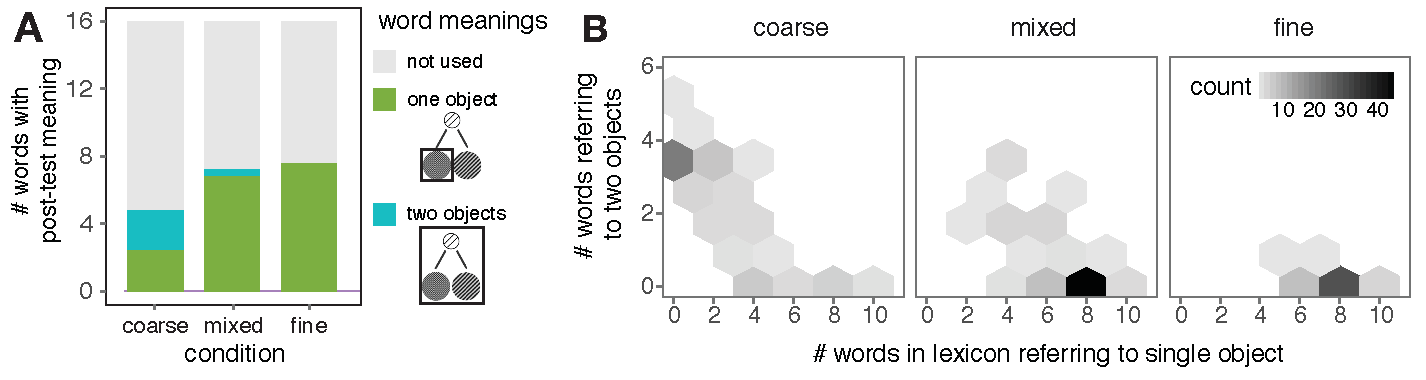
\includegraphics[scale=.7]{resultsFig_v1.pdf}
%\caption{ . (A)  (B) Diversity of terms within
%reported lexica: many participants in the coarse condition reported a mixture of abstract and specific terms.}
%\label{fig:modelresults}
%\end{figure}

%Words exist for referring at many levels of specificity: from the broadest (thing) to the most specific (Fido). What drives the emergence of these taxonomies of reference? Recent computational theories of language evolution suggest that communicative demands of the environment may play a deciding role. Here, we investigate local pragmatic mechanisms of lexical adaptation that may undergird global emergence by manipulating context in a repeated reference game where pairs of participants interactively coordinate on an artificial communication system (see Fig. \ref{fig:2018task}). We hypothesize that pairs should coordinate on conventions for specific names (e.g. Fido) when the context requires frequently making fine distinctions between entities; conversely, they should converge on a more compressed system of conventions for abstract categories (e.g. dog) in coarser contexts, even if a finer mapping would be sufficient. We show differences in the levels of abstraction that emerged in different environments (see Fig. \ref{fig:2018task}) and introduce a statistical approach to probe the dynamics of emergence. Finally, we use these data as a quantitative test for the model we proposed in Chapter 3. 

%There are \emph{many} potential ways this function could be represented in the mind at the algorithmic level. It could be derived from a store of exemplars, a set of independent prototypes for each word, a neural network embedding words and objects in a vector space, and so on \cite<see>[for a recent review of candidates]{JonesEtAl15_SemanticMemory}.

\section*{Chapter 6: How general are mechanisms across modalities?}



While linguistic communication is powerful and prevalent, research on the dynamics of adaptation in other communication modalities, including drawing \cite{GarrodFayLeeOberlanderMacLeod07_GraphicalSymbolSystems,Galantucci05_EmergenceOfCommunication,HealeySwobodaUmataKing07_GraphicalLanguageGames,TheisenEtAl10_SystematicityArbitrariness,FayGarrodRobertsSwoboda10_InteractiveEvolution} and gesture  \cite{goldin1996silence,goldin-meadow_role_1999}, is important for two reasons.
First, a core claim of the proposed hierarchical Bayesian model is that the learning and social cognition mechanisms underlying communication are domain-general.
In other words, there is nothing special about spoken or written language; any ad hoc system that we use to send messages should display similar learning dynamics.
In all cases we are trying to coordinate on meaning with other minds. 
Second, because this model also claims a critical role for background priors about what is expected to be meaningful, different communication modalities should nevertheless display certain systematic differences.
For example, the abstract tangram shapes used in Chapter 4 were hard to name but would be easy to draw.
Conversely, common objects like pieces of furniture are easy to refer to in the linguistic modality (e.g. `armchair', `lawn chair') due to strong background conventions, but hand-drawing the necessary distinctions may be costly, creating a functional need to form local conventions. 

\begin{figure}[t!]
\centering
\includegraphics[scale=0.8]{chapter6}
\caption{\small Results from the graphical reference game in Chapter 6. (A) Examples of two dyads depicting the same object over successive trials (B) Performance improves for repeated objects more than for control objects only seen at the beginning and end. (C) Drawings were harder for naive viewers to recognize in the absence of interaction history.}
\label{fig:chapter6}
\end{figure}

In \textbf{Chapter 6}, I explored the hypothesis that extended visual communication may promote the development of increasingly idiosyncratic yet effective ways of depicting objects \cite{hawkins2019disentangling}.
Specifically, I designed an interactive drawing-based reference game (i.e.~\emph{Pictionary}) similar to those used in previous chapters in which two participants repeatedly referred to targets in a context of chair images.
I examined both how their task performance and the drawings they produced changed over time (see Fig.~\ref{fig:chapter6}A).
There are three aspects of this current work that advance previous work in this modality \cite<e.g.>[]{GarrodFayLeeOberlanderMacLeod07_GraphicalSymbolSystems}.
First, I included a set of control objects that were not repeatedly drawn but only shown at the beginning and end of the interaction, allowing measurement of the specific contribution of repeated reference vs. general practice effects.
These control objects did not show the same performance gains as the repeated objects (Fig. \ref{fig:chapter6}B), suggesting that conventions were object-specific. 
In a second experiment, I measured how strongly the visual properties of drawings drive recognition in the absence of interaction history for naive viewers (the \emph{scrambled} condition), while equating other task variables (the \emph{yoked} condition).
Drawings became substantially harder for independent viewers to recognize without sharing the full interaction history (Fig. \ref{fig:chapter6}C).
\emph{Third}, I employed a convolutional neural network to quantitatively characterize changes in the high-level visual properties of drawings across repetitions \cite{simonyan2014very,FanCommon2018}---a graphical analog of the semantic embeddings used in Chapter 4.
Drawings became increasingly consistent within an interaction, but different pairs discovered different equilibria in the space of viable graphical conventions.
The strong correspondence between these results and those found using linguistic communication suggests that the same generic learning and social reasoning mechanisms may support coordination across communication modalities.

\section*{Conclusions}

The goal of my dissertation was to 
Language is not some monolithic body of knowledge that we acquire at an early age and deploy mechanically for the rest of our lives. Nor is its evolution a slow, inter-generational drift. It is a means for communication -- a shared interface between minds -- and must therefore adapt over the rapid timescales required by communication. In other words, we are constantly learning language. Not just one language, but a large variety of related languages, across every repeated interaction with every partner. 

My research program seeks to understand the core cognitive mechanisms that give rise to human social intelligence.
In pursuit of this goal, I collect rich data from naturalistic social interactions in order to infer sets of candidate mechanisms, and instantiate them in computational cognitive models that reverse-engineer the algorithmic principles of social cognition. 
In addition to making quantitative predictions that address fundamental questions in cognitive science, these models also have broader application potential toward building more socially intelligent AI.
By computationally characterizing these cognitive mechanisms, we will be better positioned to understand how interactions between individuals collectively give rise to human culture. 



%\section{\bf Acknowledgments}
%\small
%\noindent RXDH was supported by the Stanford Graduate Fellowship and the National Science Foundation Graduate Research Fellowship under Grant No. DGE-114747.

\small
\singlespacing
\bibliography{precis}
\bibliographystyle{apacite}


\end{document}  
